TODO paste in results

\section{Additive Effect Sites}

This assay uses ``dosed'' knockouts as the basis for estimation.
For these knockouts, we assume that we've already tperformed a single-site knockout screen to eliminate any non-cryptic sites from consideration.
Among remaining sites, we randomly sample $n$ and knock them out together.
You can easily imagine a dose-response curve where small doses would infrequently create detectable effects and large doses would more frequently create detectable effects.
The shape of this dose curve will depend on the underlying quantity of small effect sites and their average magnitude.
We propose to model this according to a negative binomial distribution, which models the number of coin flips that succed with probability $p$ needed to reach a number of successes $n$.
By fitting a negative binomial curve to estimate $n$ and $p$ we can estimate the mean fitness effect of additive sites ($1/n$ where 1 is the threshold of detectability) and the number of sites as $m \times p$ where $m$ is the genome length.

% Set Up Sample Genome
% Create a genome with 1,000 distinct sites, with 5% having an additive fitness effect when knocked out. Effect sizes are distributed uniformly between 0 and 0.2, relative to the detectability threshold of 1.0.

% num_sites = 1000
% distn = lambda x: np.random.rand(x) * 0.2  # mean effect size of 0.1
% additive_array = create_additive_array(num_sites, 0.05, distn)
% genome = GenomeExplicit(
%     [CalcKnockoutEffectsAdditive(additive_array)],
% )
% The true number of additive sites is

% num_additive_sites = additive_array.astype(bool).sum()
% num_additive_sites
% 50
% Choose Dose Levels
% Perform exploratory knockout experiments at a broad range of dose levels to decide the knockout doses to focus on testing.

% knockout_doses = pick_doses_extrema(
%     genome.test_knockout, num_sites, max_doses=5, smear_count=250
% )
% knockout_doses
% array([ 87, 136, 186, 236, 286])
% Estimate Additive Site Prevalence
% Do 1,000 knockout tests at each dose, fit distribution to observed sensitivity rates at each dose, and then estimate per-site effect size and num additive sites.

% est = assay_additive_naive(
%     genome.test_knockout, num_sites, knockout_doses, num_replications=1000
% )
% display(est)
% {'num additive sites': 50.0,
%  'per-site effect size': 0.1,
%  'negative binomial fit': {'r': 10,
%   'p': 0.05,
%   'fit quantiles': [0.011607600050082314,
%    0.1443781613704493,
%    0.4530475032674642,
%    0.7462911216433314,
%    0.9097429398280551],
%   'error': 0.0008510447653139157},
%  'knockout doses': array([ 87, 136, 186, 236, 286]),
%  'dose sensitivies': [0.013, 0.141, 0.43, 0.729, 0.907]}
% print("actual", num_additive_sites)
% print("estimated", est["num additive sites"])
% actual 50
% estimated 50.0

\section{Epistatic Effect Sites}

\begin{figure}
  \centering
  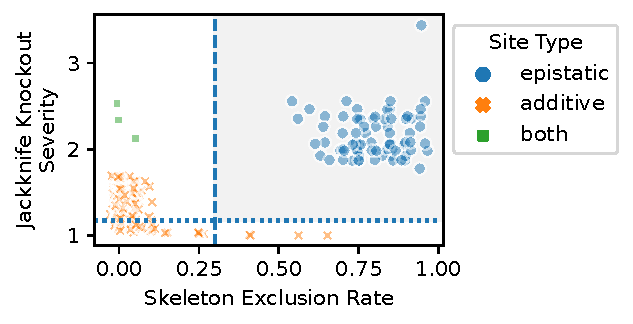
\includegraphics[width=\linewidth]{binder/teeplots/hue=site-type+style=site-type+viz=scatterplot-rect+x=skeleton-exclusion-rate+y=jackknife-knockout-severity+ext=}
  \vspace{-0.25in}
  \caption{%
    Use of knockout effect sizes and inclusion rates within ``skeletonized'' minimal viable genomes to distinguished small-effect and epistatic genome sites.
  }
  \label{fig:epistatic}
  \vspace{-0.25in}
\end{figure}


This assay uses minimal viable genomes, ``skeletons,'' as the basis for estimation.
Repeated stochastic successive knockout process until no more sites can be removed to generate a sample of skeletons.
The intuition is that sites that appear infrequently in skeletons but not others are epistatic.
However, additive small-effect sites will also appear sometimes appear outside skeletons.

We can use knockout effect size to differentiate these cases.
For this procedure, we iterate through the skeleton and do ``jackknife'' single site knockouts.
If the marginal knockout effect size of this site is very small, then it is probably an additive site.
If the marginal knockout effect of the site in the skeleton context is big, it is probably an epistatic effect site --- with the rest of its redundant sites already excluded from the skeleton.
Figure \ref{fig:epistatic} shows this distinction.

% Create Sample Genome
% Create a genome with 4,000 distinct sites.

% Let 5% of sites have an additive knockout fitness effect below detectability threshold (uniform between 0 and 0.7 fitness effect).

% Assign 20 sets of epistatic effects, with 5 sites per set. Apply a set-specific fitness penalty between 0.7 and 1.6 when all sites in a set are knocked out.

% Fitness 1.0 is considered the threshold for detectability

% neutral      3706
% additive      195
% epistasis      94
% both            5

% "Skeletons" are minimal sets of genome sites that maintain wile-type fitness. Skeletons can be generated by sequentially removing sites from the genome, until no further sites can be removed without detectably reducing fitness.

% Sample 20 skeletons.

% "Skeletons" are minimal sets of genome sites that maintain wile-type fitness. Skeletons can be generated by sequentially removing sites from the genome, until no further sites can be removed without detectably reducing fitness.

% Sample 20 skeletons.

% Use Skeleton Jackknifes to Differentiate Epistasis versus Additive Sites
% Our goal is to isolate epistatic sites and then count them up.

% Do this by setting thresholds for skeleton exclusion frequency and jackknife knockout severity, then counting sites that exceed both thresholds.

% First, set the skeleton exclusion frequency threshold at 0.3. Then, look at all points excluded less than 30% of the time. Take the 20th percentile of these sites' jackknife knockout severities. This is the jackknife knockout severity threshold.

% Then, count sites that exceed both thresholds.

% est = assay_epistasis_naive(
%     df_skeletons,
%     exclusion_frequency_thresh=0.3,
%     jackknife_severity_thresh=0.2,
% )
% est
% {'num epistasis sites estimate': 80,
%  'exclusion frequency cutoff': 0.3,
%  'jackknife severity cutoff': 1.1739066427089908}
% For comparison, the actual count of epistasis sites is

% df_genome["site type"].value_counts()["epistasis"]
% 94
% This estimate could probably be improved with mark-recapture methods as used in the "agnostic" methods.

% Note the presence of very small-effect additive sites (i.e., low jackknife knockout severity) with high exclusion rates. This is why we need jackknife severity to identify epistatic sites.

\section{Any Effect Sites}

Skeletons can be put to another use to try to directly estimate the number of sites that have any fitness effect.
Reframed, skeletoniz.
Any site that has a fitness benefit should, in principle, potentially appear within a skeleton.
Skeletons randomly sample from among these sites.
Framed this way, sampling a skeleton genome is not unlike a trap sampling study used by wildlife biologists.
Extensive, well-developed mathematics exists around this problem.
Such math will need to be careful to account for ``shyness'' --- uneven probability for some sites appearing in a skeleton.
We propose to use the Burnham-Overton estimation procedure.
We give it a distribution of, among the sites that appeared within skeletons, the number of skeletons they appeared in and it gives us a total population estimate

% # Burnham, Kenneth P., and W. Scott Overton.
% # "Robust estimation of population size when capture probabilities vary among
% # animals." Ecology 60.5 (1979): 927-936.
% # https://doi.org/10.2307/1936861

% Create Sample Genome
% Create a genome with 10,000 distinct sites.

% Let 4% of sites have a knockout fitness effect below detectability threshold. Effect sizes are distributed uniformly between 0 and 0.7, relative to the detectability threshold of 1.0.

% Add 40 epistatic sets, each with 4 sites. Fitness consequences of magnitudes between 0.7 and 1.6 occur when all sites within an epistatic set are knocked out.

% Overlap is allowed --- n individual sites may have both additive and epistatic effects.

% num_sites = 10000
% distn = lambda x: np.random.rand(x) * 0.7
% additive_array = create_additive_array(num_sites, 0.04, distn)
% epistasis_matrix = create_epistasis_matrix_disjoint(num_sites, 40, 4)
% genome = GenomeExplicit(
%     [
%         CalcKnockoutEffectsAdditive(additive_array),
%         CalcKnockoutEffectsEpistasis(epistasis_matrix, effect_size=(0.7, 1.6)),
%     ],
% )

% neutral      9445
% additive      395
% epistasis     155
% both            5
% Name: site type, dtype: int64

% How many functional (i.e., non-neutral) sites are there?

% num_functional_sites = (df_genome["site type"] != "neutral").sum()
% num_functional_sites
% 555
% Perform Skeletonizations
% "Skeletons" are minimal sets of genome sites that maintain wile-type fitness. Skeletons can be generated by sequentially removing sites from the genome, until no further sites can be removed without detectably reducing fitness.

% How many unique sites show up in any skeleton? (i.e., num sites with direct evidence of functionality)

% np.any(
%     (~skeletons.astype(bool)),
%     axis=0,
% ).sum()
% 504
% Estimate Number Functional Sites
% The skeletonization process can actually be interpreted as a mark-recapture experiment. Just like field researchers counting rabbits, we can estimate the total population of functional sites from the rate at which we "re-capture" specimens. (Here, "re-capture" means that a site is included in more than one skeleton.)

% Note that statistics taking into account bias in capture probability (aka "trap shyness") are necessary. This implementation uses a nonparametric jackknife estimator due to Burnham and Overton (see source code for details).

% assay_agnostic_naive(df_skeletons)
% {'num sites estimate': 558.3499999999999,
%  'num sites 95% CI': (533.2059805122569, 583.4940194877429)}
% For comparison the actual number of functional sites is

% num_functional_sites
% 555
